\chapauth{Mortonic}
\chapter{The Very Hungry Luke Bavarius}





In the light of the moon, a little egg lay on a leaf.



One sunday morning the warm sun came up and pop! Out of the egg
came a tiny and very hungry private detective, Luke Bavarius.



He started to look for some food.



On Monday he ate through some black culture. But he was still
hungry.



On Tuesday he ate through two Berettas. But he was still
hungry.



On Wednesday he ate through three piles of vomit. But he was still
hungry.



On Thursday he ate through four sparkly Bavarius badges. But he was
still hungry.



On Friday he ate through five gooooooold rings. But he was still
hungry.



On Saturday he ate through an entire Baconator! That night he had
stomach-ache!



The next day was Sunday again. Luke ate through one nice green
leaf, and after that he felt much better.



Now he wasn't hungry anymore --- and he wasn't a little private
detective any more. He was a big fat private detective.



He built a small house, called a cocoon, around himself. He stayed
inside for more than two weeks. The he nibbled a hole in the cocoon
and pushed his way out{\ldots}



He was a horrid reflection!



%% He then began to read approximately 500 words of the Bible:



%% Genesis



%% 1 First God made heaven \& earth 2 The earth was without form
%% and void, and darkness was upon the face of the deep; and the
%% Spirit of God was moving over the face of the waters. 3 And God
%% said, ``Let there be light''; and there was light. 4 And God saw that
%% the light was good; and God separated the light from the darkness.
%% 5 God called the light Day, and the darkness he called Night. And
%% there was evening and there was morning, one day. 6 And God said,
%% ``Let there be a firmament in the midst of the waters, and let it
%% separate the waters from the waters.'' 7 And God made the firmament
%% and separated the waters which were under the firmament from the
%% waters which were above the firmament. And it was so. 8 And God
%% called the firmament Heaven. And there was evening and there was
%% morning, a second day. 9 And God said, ``Let the waters under the
%% heavens be gathered together into one place, and let the dry land
%% appear.'' And it was so. 10 God called the dry land Earth, and the
%% waters that were gathered together he called Seas. And God saw that
%% it was good. 11 And God said, ``Let the earth put forth vegetation,
%% plants yielding seed, and fruit trees bearing fruit in which is
%% their seed, each according to its kind, upon the earth.'' And it was
%% so. 12 The earth brought forth vegetation, plants yielding seed
%% according to their own kinds, and trees bearing fruit in which is
%% their seed, each according to its kind. And God saw that it was
%% good. 13 And there was evening and there was morning, a third day.
%% 14 And God said, ``Let there be lights in the firmament of the
%% heavens to separate the day from the night; and let them be for
%% signs and for seasons and for days and years, 15 and let them be
%% lights in the firmament of the heavens to give light upon the
%% earth.'' And it was so. 16 And God made the two great lights, the
%% greater light to rule the day, and the lesser light to rule the
%% night; he made the stars also. 17 And God set them in the firmament
%% of the heavens to give light upon the earth, 18 to rule over the
%% day and over the night, and to separate the light from the
%% darkness. And God saw that it was good. 19 And there was evening
%% and there was morning, a fourth day. 20 And God said, ``Let the
%% waters bring forth swarms of living creatures, and let birds fly
%% above the earth across the firmament of the heavens.'' 21 So God
%% created the great sea monsters and every living creature that
%% moves, with which the waters swarm, according to their kinds, and
%% every winged bird according to its kind. And God saw that it was
%% good. 22 And God blessed them, saying, ``Be fruitful and multiply
%% and fill the waters in the seas, and let birds multiply on the
%% earth.'' 23 And there was evening and there was morning, a fifth
%% day. 24 And God said, ``Let the earth bring forth living creatures
%% according to their kinds: cattle and creeping things and beasts of
%% the earth according to their kinds.'' And it was so. 25 And God made
%% the beasts of the earth according to their kinds and the cattle
%% according to their kinds, and everything that creeps upon the
%% ground according to its kind. And God saw that it was good. 26 Then
%% God said, ``Let us make man in our image, after our likeness; and
%% let them have dominion over the fish of the sea, and over the birds
%% of the air, and over the cattle, and over all the earth, and over
%% every creeping thing that creeps upon the earth.'' 27 So God created
%% man in his own image, in the image of God he created him; male and
%% female he created them. 28 And God blessed them, and God said to
%% them, ``Be fruitful and multiply, and fill the earth and subdue it;
%% and have dominion over the fish of the sea and over the birds of
%% the air and over every living thing that moves upon the earth.'' 29
%% And God said, ``Behold, I have given you every plant yielding seed
%% which is upon the face of all the earth, and every tree with seed
%% in its fruit; you shall have them for food. 30 And to every beast
%% of the earth, and to every bird of the air, and to everything that
%% creeps on the earth, everything that has the breath of life, I have
%% given every green plant for food.'' And it was so. 31 And God saw
%% everything that he had made, and behold, it was very good. And
%% there was evening and there was morning, a sixth day. 

\begin{figure}[b]
  
  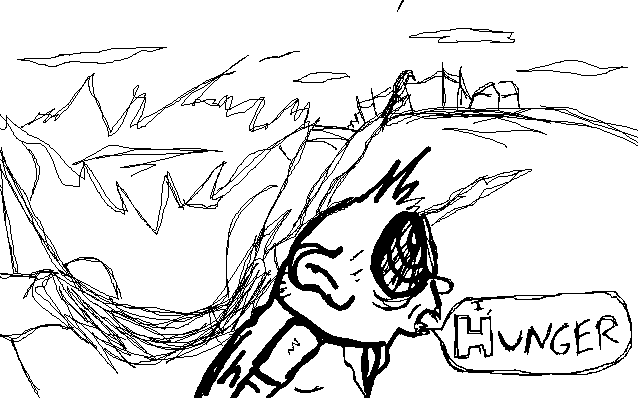
\includegraphics[width=\textwidth]{art/Lord_Humongus-Hungry.png}
  \caption{{\em Hunger} by Lord Humongus}
  
\end{figure}

